\documentclass[12pt]{article}
\usepackage{amsfonts, amsmath, fancyhdr}
\usepackage{algorithm}
\usepackage[noend]{algpseudocode}
\usepackage{bbm}
\usepackage{csquotes}
\usepackage{graphicx}
\usepackage{url}

\pagestyle{fancy}

\topmargin = -0.8 in
\oddsidemargin = 0.0 in
\evensidemargin = 0.0 in
\textheight = 9 in
\textwidth = 6.5 in

\newtheorem{theorem}{Theorem}   
\newtheorem{result}{Result}
\newtheorem{definition}{Defintion}  

\algnewcommand\algorithmicforeach{\textbf{for each}}
\algdef{S}[FOR]{ForEach}[1]{\algorithmicforeach\ #1\ \algorithmicdo}
\renewcommand{\algorithmicensure}{\textbf{Result:}}

\begin{document}

\lhead{ } \chead{ } \rhead{ } \lfoot{ } \cfoot{\sf -- page
\thepage~  of 20 --  } \rfoot{ }                                            %            <=====   PAGE NUMBERING NEEDS TOTAL

\title{\bfseries NYC Subway Social Distancing Risk Analysis}
\author{CSCI - 740 Computer Modeling and Simulation\vspace*{0.5em} \\ \vspace*{0.5em} Group 1:\\
Alex Washburn, Andrew Lee, Kamil Sachryn,  Chuanyao Lin, Ye Paing
}
\date{Fall 2020}

\maketitle

\begin{abstract}
	We describe a model to simulate a 24-hour cycle of a subway line and track the transmission of a virus between passengers within the train cars.
	Parameters of the model are defined to represent NYC MTA's L subway line and the virus to behave as SARS-CoV-2.
	We measure the ratio of passengers without the virus which have the virus transmitted to them during their trip to the total number of passengers without the virus as the random variable of our simulation.
	A hypothesis, control, and two interventions are described for lowering the virus transmission between passengers.
	We discuss implementation details, the variance reduction techniques applied, and the intervention outcomes of our simulation.
\end{abstract}

\clearpage

\section{Executive Summary}

The spread of SARS-CoV-2 and COVID-19 are a rampant public health crisis.
Policy guidelines and research regarding risk and transmission are still emerging, though most revolve around social distancing and face covering to minimize the spread of particulate matter between individuals.
However, these policies may have their efficacy degraded in situations where individuals are forced into close proximity.
One such situation is public transit via subway.
We propose simulating the subway train environment to quantify the risk of virus transmission under different circumstances.
The research question our simulation aims to answer is the following:


\begin{displayquote}
\emph{``How do different arrival rates of the trains and passengers impact the virus transmission risks of passengers for the duration of their subway ride?''}
\end{displayquote}

The one goal of our project is to create a model which strikes an acceptable balance between accurately modeling the physical and epidemiological conditions of a subway line while preserving computational efficiency.
Another goal is to produce actionable policy recommendations involving possible operational changes to the subway.
Using the current and pre-COVID-19 MTA subway data for arrival rates of trains and passengers, and what we know about current COVID-19 infection rate and prevention method, implement a model to simulate the novel transmissions of passengers (spreading the virus to a passenger who previously did not have the virus) that passes through the subway system for an average day, to determine the transmission risks for passengers.
We aim to use the simulation to study the expectation of ratio of novel transmissions that occurs within our simulation for various arrival rates of trains and passengers.
By doing so, we hope to provide a recommendation of train and passenger arrival rates to the MTA that would help with our current efforts reduce the transmission of SARS-CoV-2 and to combat COVID-19.

The findings of our simulation show that the increased subway trains have a moderate to minimal impact on the transmission of the virus, depending on the circumstances.
However, our simulation shows that throttling passenger admittance to the subway system has a moderate to a significant impact on reducing the transmission of the virus.
Our recommendations to the MTA are as follows:


\begin{displayquote}
	Assign at least one MTA employee per set of turnstiles entering a subway line.
	Monitor the number of passengers entering each subway station via the real-time turnstile data.
	Keep a counter of the of passengers in the station visible to the MTA station staff.
	When a train departs from the station, reset the counter to 0.
	When 100 passengers have entered a station, and the counter reads 100, have the assigned MTA employees stop admitting new passengers through the turnstiles until after the next train departs and the counter has reset.
	The above represents a cost-effective policy for reducing the transmission of the virus with the subway trains by 40\% to 98\%.
\end{displayquote}


\clearpage

\section{Introduction and Background}
\paragraph{}
The subway system within New York City is an essential service which transports over a million people daily even during an epidemic\cite{mta}, but the New York Subway system may be dangerous to ride with little ways to socially distance while on the train.
To better understand and mitigate the risks of viral spread on the Subway system, this project aims to simulate and gain insight on how train and passenger arrival rates affect the spread of COVID-19.
Using this data it may be possible to further reduce the risk of infection for the residents of New York via changing the arrival rates of trains or limiting the maximum number of people queued at a station.

Over 37\% of New York's workers use the subway to commute to their workplace \cite{ridership_census}. This figure alone makes the subway system an integral part of New York City's workforce.
Such a large percentage of the city's population leads to very high infection rates as people are unable to properly socially distance within each subway car, leading to more and more people becoming infected and in turn infectious to other people.
Due to the vast spread of the virus, and it having quickly become a pandemic, the ridership of the New York City subway shrunk by 70\%\cite{mta} which improved the chances for each remaining commuter, but it did not completely negate the risk of infection. To further mitigate the chance of infection, further measures must be taken.

Since the discovery of the disease in New York City more than 20,000 cases have been discovered, and the number is constantly rising\cite{disease_numbers}.
The virus itself is a part of the Severe Acute Respiratory Syndrome family of viruses, otherwise known as SARS.
This virus is the cause of the COVID-19 disease, occurring between two and fourteen days after initial infection.
Part of the danger of COVID-19 is that the viral load of the virus, the amount of the virus within the host's system, is at it's greatest point half a day before the onset of symptoms.
Such a high concentration of the virus before the onset of symptoms causes the disease to be much more severe in comparison to other similar diseases such as the original SARS virus, which had it's peak viral load 10 days after the onset of symptoms.\cite{viral_load}

COVID-19 is dangerous and highly virulent for several reasons, and required constant attention and precautions to avoid infection.
COVID-19 is a disease cased by the virus SARS COVID-II, a member of the SARS family of viruses, causing respiratory issues.
The disease itself and the virus are separate, which means that even a person who does not display any symptoms of the disease is capable of spreading the virus to other people.
This is especially dangerous as the virus is able to spread in medium much smaller than previous SARS viruses, specifically it is able to spread in tiny saliva droplets let out during speech, rather than only bigger ones released during sneezes or coughs.
Further differences from previous SARS viruses include an adhesion rate to cell membranes that is ten times higher, leading to far fewer of the virus needing to enter a system in order to begin multiplying.
Lastly, the virus has an extremely long lifespan outside of a body, being able to remain active and infectious for up to 72 hours on plastic and steel surfaces.
To account for these issue, it is necessary to think of each person as 'contagious' or 'non-contagious' rather than whether or not the person is infected, as simply touching another person may lead to infection from a person who is not infected, but contagious. 

To avoid contact with contagious people as well as inanimate sources of contagion, as well as viruses floating in the air, several steps must be taken.
In order to minimize the chance of contracting the virus from another contagious person one must remain outside of close contact with any other person.
Close contact is defined as spending 15 minutes within 6 feet of a contagious person within the time period of one day \cite{distancing_recommendations}.
The six foot distancing recommendation is supplemented by wearing masks and other protective gear in order to limit the chances that the virus can infect another person via saliva droplets, as well as by washing hands, and any surface that touched anything else, in order to remove the virus and stop it's spread via touch. 

%Social distancing can be difficult on an individual subway car, with the 6 foot figure being difficult to implement in a cramped place, especially during high congestion times. The typical L-Line train car, the R143, has an area of 54.65\(m^2\) (18.35m x 2.98m)\cite{dimensions}. In order to fit the average size of a US citizen of 0.16m \cite{body_size} on the R143 train and maintain a 6 foot radius of separation between people we could only fit a theoretical maximum of 25 people on each train, accounting for the sides of the train as well as the four corner of a train car, a much smaller number than the 256 it is capable of transporting at one time. Going above this value would cause a guaranteed unsafe area. 

Calculating the optimal rate of arrival of trains and passengers can lead to both lower infection rates as well as making the subway system more economically efficient. 
With a random rate of infection, rate of passenger generation, and a fixed train schedule we are able to accurately model the system as a whole, and through many replications come to a conclusion on it's safety.
As the number of trains increases we are able to create more safe spaces for each passenger, but at the same time costs would greatly increase. 
In order to reach an equilibrium we must find a value where the expected number of transmissions is as low as possible while remaining viable for the company.
To accomplish this we are able to test different combinations of parameters, altering the model in order to find the most efficient solution. 

The goal of this project is to determine the optimal arrival rate of both passengers at each station, as well as the frequency of trains along the L-Line.
The arrival rate of people at each station is different, dependent on both the popularity of the station in general as well a the current time of day.
A station is likely to be the most popular when people leave for work, as well as when they come back, ending up in two periods of greatly increased traffic and chance of infection via being unable to socially distance.
Secondly, the amount of trains during this time must be increased, while the amount of trains during off-hours can be decreased to save any costs incurred by lowering the amount of trains during peak hours.
These changes would be based on the project's simulation of different sets of variables, measuring the benefits and drawbacks of each and coming to a final conclusion.

\section{Methodology}
In this section, we will go over in depth our techniques and methodology for building the different parts of our simulation.
These includes how we gather data to support our simulation, generating the arrival of passengers and trains, placing passengers on the trains and detecting if social distancing is observed, and how we move the trains and passengers through the system for the duration of our simulation.

To simulate our subway line, we will start feeding trains into the system at one end of the line, and terminate them at the other end (last stop) of the line.
This implies that for our simulation, we will only be simulating the train going in one particular direction.
In the case of the L line that we are simulating, we can either run the simulation from Brooklyn to Manhattan, or in the opposite direction of Manhattan to Brooklyn.
The trains will then move deterministically through the stations, and at each station, the passengers will disembark from the train cars, then the passengers who are on the queue at that particular station will embark onto the train car from the queue. We will be simulating multiple train cars, with a max capacity for each train car (more details on modeling the space in the train car below).

For the majority of our data, we reference the MTA websites and related sources to come up with train and passenger arrival rates for our simulation.
For the project, we had settled on simulating the L train line, as it was one of the few lines in the MTA system that ran in a linear, bi-directional manner.
Meaning, for the purpose of our simulation, we will not consider transfers from other subway lines, and also different line configuration based on time of day (for example some lines have different stops during rush hour). 

\subsection{Model Overview}

Our model has a discrete time parameter $t \in [0, T] \subset \mathbb{N}$, with the range $[0, T]$ representing 24-hour cycle of the subway line.
For our simulation we choose one minute time resolution for $t$ ranging for $[0, 1440]$.
However, the model could easily be re-parameterized to work with finer or coarser temporal quanta.

Initially started out with a naive tick-based implementation, but as we gathered data and finalized on our research question and goals of the project, we had decided to switch over to a retrospective model, allowing us to retroactively determine the passenger arrival rates between trains. For a more detailed description, see Algorithm \ref{Alg:main-loop} in the appendix.

Our model specifies a ``rate of spread'' parameter $r$, representing the probability of transmitting the virus for each quantum of time that a passenger is within 1.7 meters of another passenger with the virus.
The selection of this $r$ value in our simulation is set to $r=\frac{1}{15}$ based on U.S. CDC's guidelines. They label high-risk "Close Contact" with any individual to be anything more than the duration of 15 minutes. Using this as our mean time of transmission of the geometrically distributed "time until transmission" variable, the probability of success per minute was derived to be $0.0666$.

%a contact tracing and testing study conducted in Guangzhou, China \cite{guangzhou-study}. 

Each passenger has a probability $c$ of entering the subway system with the virus.
We call these passengers ``initially contagious passengers.''
We call a passenger who entered the subway system without the virus an ``initially non-contagious passenger''.
When an initially non-contagious passenger has the virus transmitted to them, we call this event a ``novel transmission'' and we also call this passenger a ``contagious passenger'' (though not an \emph{initially} contagious passenger).

The model output is the ratio of the total number of novel transmission events that occurred to the total number of initially non-contagious passengers.
The output of the model is a random variable in the range $[0, 1]$.
This expectation of the random variable represents the probability that an initially non-infection passenger will have the virus transmitted to them during their ride.
Our simulations will replicate running the model, taking the mean of the outputs in order to determine the expectation of the random variable.

$$ X = \frac{\text{novel transmissions}}{\text{initially non-contagious passengers}} $$

\subsection{The Subway Line}

Our model specifies as a parameter a sequence of $n$ stations $\mathcal{S} = \{ S_0^q, S_1^q, ... , S_{n-1}^q \}$ representing our subway line with a maximum queue length $q$.
We denote that $S_0^q$ is the ``first'' station of the subway line, at which trains will arrive and being their transit through the subway line. We also denote $S_{n-1}^q$ as the ``last station'' of the subway line, at which trains are removed from the model.
Additionally we require a reflexive and transitive relation $\mathcal{D} : \mathcal{S} \times \mathcal{S} \mapsto \mathbb{Z}$ which measures the distance between stations as a multiple of the quantum $t$.
Note that $\mathcal{D}$ is not a symmetric relation, as it represents the directed distance between stations.
A negative distance value of $\mathcal{D}(S_i^q,S_j^q)$ implies $S_j^q$ is ``before'' $S_i^q$ in the subway line and would require going in the opposite direction of the subway line's transportation direction to reach $ S_j^q$.
For our simulation, we reference the MTA's website for a list of L line subway stations and their distances from each other, see Figure \ref{L-line-map}.

\begin{figure}[h]
	\centering
	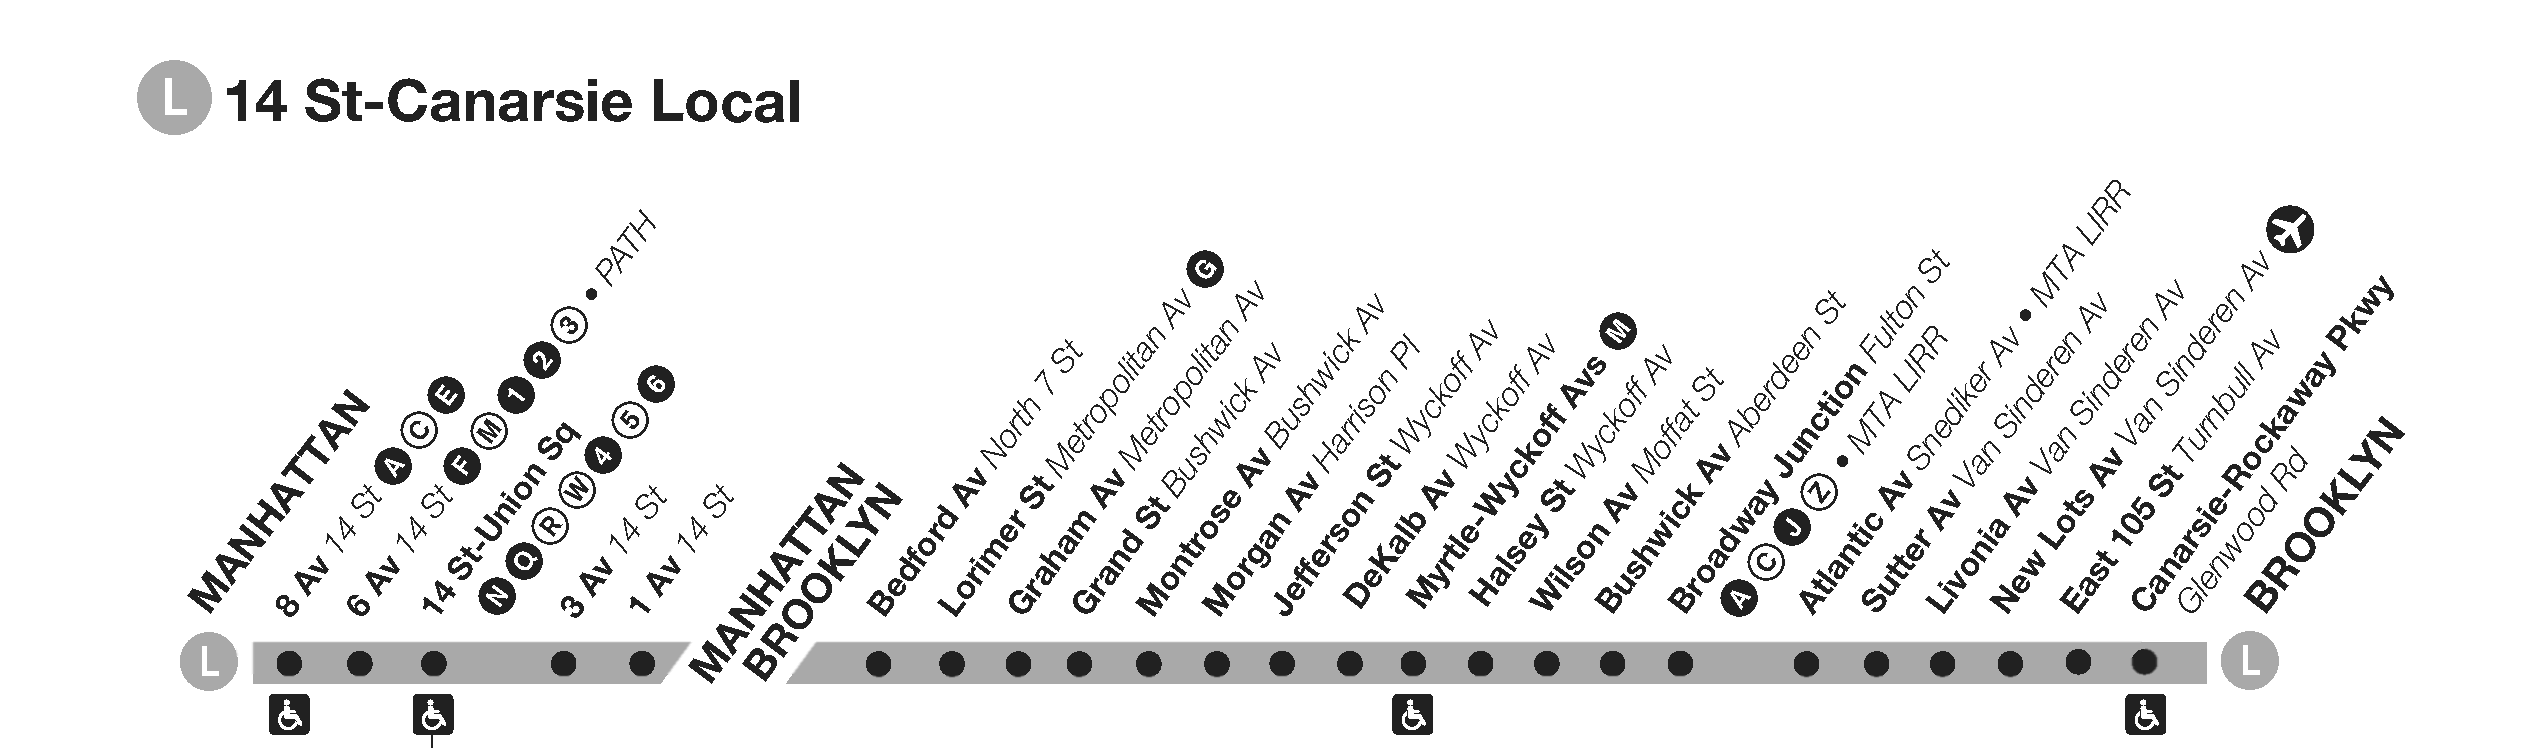
\includegraphics[scale=.80]{./figures/route-l-map.png}
	\caption{MTA Subway stops for L line}
	\label{L-line-map}
\end{figure}

\hfill \newline


\subsection{Passenger Arrival Rate and Departure Weights}

Our model specifies as a parameter a sequence of $n$ arrival rates of passengers $\{ \lambda_0(t), \lambda_1(t), ... , \lambda_{n-1}(t) \}$ and a sequence of $n$ departure weights of passengers $\{ \mu_0(t), \mu_1(t), ... , \mu_{n-1}(t) \}$ which may vary based on the current time $t$ of the simulation.
Each arrival rate $\lambda_i(t)$ corresponds to the Poisson process of passengers enqueuing at station $S_i^q$.
Each departure weight $\mu_i(t)$ correspond to the proportion of all passengers arriving at station $S_i^q$ which depart at $S_i^q$ rather than departing at another station.
We can construct from the $\mu$ values an origin-destination matrix $P_{ij}(t)$ which defines the probability of passenger entering the subway system at station $S_i^q$ having the probability of departing at station $S_j^q$:

\[ P_{ij}(t) = \frac{\mu_j(t)}{\sum_{k=0}^{n-1} \;\mathbbm{1}_{\mathcal{D}(S_i^q, S_k^q) > 0}\; * \; \mu_k(t)} \]

Due to the linear nature of the subway line, the resulting matrix $P_{ij}(t)$ will be an upper triangular matrix with zeroes along the diagonal. It is also worth noting for the ``last'' station $S_{n-1}^q$, for all $t \in [0, T]$, $\lambda_{n-1}(t) = 0$ and $P_{(n-2)(n-1)}(t) = 1$. 

By allowing the $\lambda$ and $\mu$ values to vary with respect to $t$, we can model more precisely the different usage of the subway line throughout the daily cycle. 
We collected data on subway arrival rates at different times of the day.
The MTA provided data\cite{arrival_rate} in six time intervals, \texttt{00:00} (midnight) to \texttt{04:00}, \texttt{04:00} to \texttt{08:00}, \texttt{08:00} to \texttt{12:00}, \texttt{12:00} to \texttt{16:00}, \texttt{16:00} to \texttt{20:00}, and \texttt{20:00} to \texttt{00:00}.
For each interval of time, we model each station $S_i^q$ as having a homogeneous Poison process with intensity $\lambda_i(t)$ where $t$ is in the time interval.
For example, given the time window \texttt{00:00} to \texttt{04:00}, and our one minute resolution of quanta for $t$, $S_i^q$ will have a homogeneous Poisson process with intensity $\lambda_i(t)$ for all $t \in [0, 240]$.
For the specific weekday ridership of the station n, we can calculate the number of arrivals of passengers in one time interval by summing all of the new turnstiles entries in that station. For example, the number of passengers arriving at the station n from 0:00 AM to 4:00 AM on that specific weekday will be the number of entering passengers of the turnstile j on 4:00 AM minus the number of passing passengers of the turnstile j on 0:00 AM for all j turnstiles in that specific station. So, we can get the average weekday ridership of the different time intervals(every 4 hours) of each station from the calculated weekdays ridership. Each arrival rate $\lambda_i(t)$ will be the average weekday ridership divided by 240(mins) based on the different time intervals. However, since some stations contain multiple lines, we're not able to know which directions will the passengers take after they entering the station. Therefore, we make a simplifying assumption that the number of passengers entering a station will be evenly divided between the number of available subway lines and each nth portion of the number of passengers will take one of the n subway lines. For example, a station with 2 subway lines will have their $\lambda_i(t)$  divided the by 2 to indicate 2 different directions, then if a station contains multiple lines, we'll keep dividing $\lambda_i(t)$ by the number of lines.

\subsection{Passengers}

Our model lazily draws from an infinite sequence unique passengers which arrive at stations based on the station's Poisson process. Each passenger $P_i$ arriving at station $S_i^q$ is given a ``destination station'' annotation  $S_k^q$, such that $\mathcal{D}(S_i^q, S_j^q) > 0$ (a negative distance implies the destination is in the opposite direction that the subway line is traveling).
Additionally, each passenger has a probability $c$ of entering the subway system with the virus. Lastly, each passenger has a ``time to transmission'' annotation which is sampled from a geometric distribution with $p=r$, where $r$ is the rate of spread as defined above.

Passengers queue at their source station $S_i$, until a train arrives at $S_i$, in which case passengers will disembark from the train first (making room for passengers at $S_i$ to embark) before passengers on the station queue will embark the train.

\subsection{The Trains}

Our model specifies as a parameter a sequence of $m$ train arrivals $\tau = \{ t_0, t_1, ... , t_m \} \subset [0, T]$, representing the times at which each train arrives at the first station $S_0^q$.
Each train will contain one or more cars in which $0$ to some maximum capacity $M$ passengers can ride within.

For our simulation, we reference the MTA's website for the arrival times of the L line, see Figure \ref{train-schedule}.
We note the MTA states that the L line runs with 8 subway cars per train so we create 8 empty subway cars for each new train entering the simulation. We also used the manufacture's specifications of the R143 New Technology Train cars built by Kawasaki Rail Car Company for the dimensions and maximum capacity $\Psi=258$.

\begin{figure}[h]
\centering
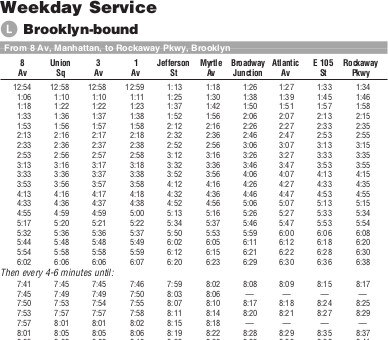
\includegraphics[scale=1.0]{./figures/l-line-scheule-snip.png}
\caption{MTA L line train schedule}
\label{train-schedule}
\end{figure}

\subsection{Modeling Subway Cars and Social Distancing}
Initially, we simply had a naive 2-dimensional grid that represented the max number of passengers that can fit safely (observing social distancing) into a subway car.
After much discussion and consultation, we realize that this might not accurately represent the transmission rate between passengers on the subway. We considered placing passengers at random $(X,Y)$ coordinates within the space of a subway car and calculating the euclidean distance between passengers.
This however, proved to be computationally expensive, requiring $\mathcal{O}(P^2)$ comparisons, where $P$ is the number of passengers in the subway car.
Thus we had decided to move towards a hexagonal grid layout of the subway car that allows for an efficient approximation of measuring euclidean distance with all the efficiency benefits of a discrete representation.

\begin{figure}[h]
	\centering
	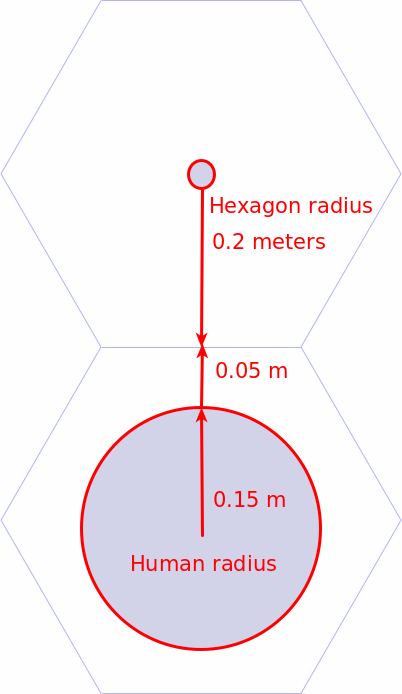
\includegraphics[scale=.30]{./figures/two-hex2.png}
	\caption{Hexagon cell of the hex grid}
	\label{hex-cell-pic}
\end{figure}

We calculated that average American body's cross-section to be roughly $1.5$ meters in radius.
We defined the hexagon radius of our grid to be $0.2$ meters, as even on a packed subway car, each passenger requires a minimal amount of space surrounding them to allow themselves and others to maneuver with the subway car, see Figure \ref{hex-cell-pic}
Given the manufacturer's specifications of the R143 New Technology Train cars, each subway car has a length of $18.35$ meters and a width of $2.98$ meters.
To model these interior dimension with hexagons of $0.2$ meter radius, we construct a $46 \times 8$ hexagonal grid, see Figure \ref{hex-grid-dimensions}.
With this construction, the hexagonal grid has a length of $18.4$ meters and a width of $3$ meters, which very closely models the actual train car dimension. 

\begin{figure}[h]
	\centering
	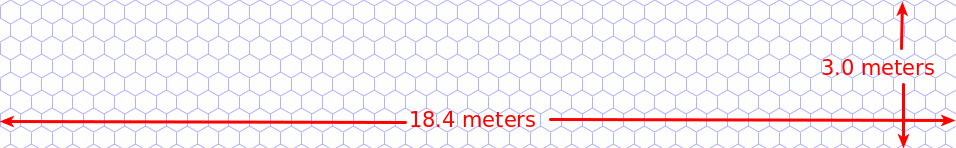
\includegraphics[scale=.45]{./figures/hex-train-dims.png}
	\caption{Subway car modeled in hex grid}
	\label{hex-grid-dimensions}
\end{figure}

%\hfill \newline
With the grid system in place, we can now easily calculate if two passengers are socially distanced by simply counting the hexes in between the two passengers.
We calculated that two passengers being 4 hexes apart (that is, 3 hexes between them) represents $1.3$ meters of separation, which is not considered social distancing.
However two passengers being 5 hexes apart, which represents about $1.7$ meters of separation, is the minimum required amount of hexes needed between passengers to be considered safely socially distanced for our simulation, see Figure \ref{social-distance-measure}.
This implies that a train car can hold 24 passengers at max, while being safely socially distanced, see Figure \ref{social-distance-full-grid}.

\begin{figure}[h]
	\centering
	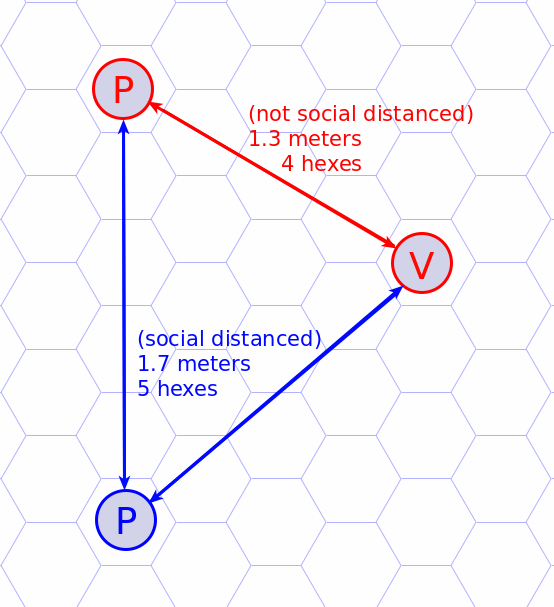
\includegraphics[scale=.35]{./figures/hex-counting.png}
	\caption{Social distance calculation and optimal passenger layout}
	\label{social-distance-measure}
\end{figure}

How well does this model the reality of social distancing in the car?
Well, first, we had to acquire some fundamental data to build our theoretical analysis. The previously mentioned average American body’s cross-section of $0.16m$ was calculated from a 17 year Body Measurement Research Study conducted from 1999 to 2016. We tried to simulate a fit of the simplified human body circles within the 2-dimensional floor cross-section of the R143 New Technology Train car layout($54.683m^{2}$). The human bodies were also given a $3ft$ (or $0.9m$) of extra radial distance, creating a “bubble” for one individual human body to have a radius of 0.9 + $0.16m$, which was $1.06m$. The assumption that human bodies are perfect circles are obvious not an exact representation of reality but it was implemented as one of the simplifications within our model as the human body cross-section is the minority portion of our individual bubbles. The $3ft$ of extra radius outside the human body was determined to establish a minimum $6ft$ socially distanced radius between 2 human individuals at any time, given that 2 different bubbles cannot overlap. Before fitting this one the subway car area, a few details about actual human placement behavior in NYC subway cars had to be noted. First was that a person normally seeks out to either sit or stand on the edge or the corner of the subway car, reducing their effective bubble area to about half for edge cases, and a quarter for corner cases. Taking these information into account, we aligned the human body bubbles along the walls and corner first, and then tried to placed the rest of the bubble in the remaining area left in the middle. This resulting number of maximum passengers that one subway car can hold where everyone is safely socially distanced was 25. This seems to closely match the number that we achieved within our hexagonal grid simulation, which was 24. 
\begin{figure}[h]
	\centering
	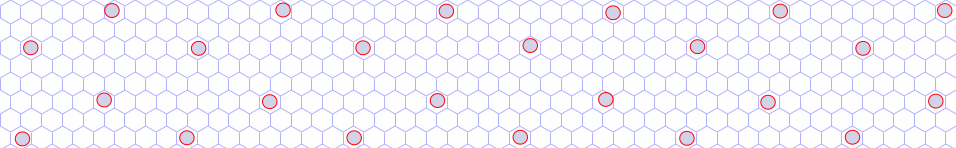
\includegraphics[scale=.45]{./figures/hex-train-full-safe.png}
	\caption{Social distance calculation and optimal passenger layout}
	\label{social-distance-full-grid}
\end{figure}

\subsection{The Embarking and Disembarking Process}

\begin{figure}[h]
\centering
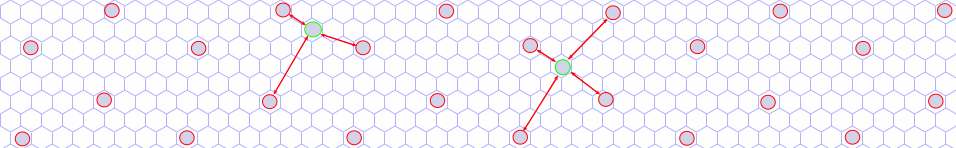
\includegraphics[scale=.45]{./figures/hex-train-full-unsafe.png}
\caption{Social distance calculation when over the ``safe'' capacity}
\label{social-distance-unsafe-car}
\end{figure}

Once a train arrives at a station, passengers that embark the train will try and position themselves in the optimal social distancing configuration as seen in Figure \ref{social-distance-full-grid}.
If however, there are more than 24 passengers (max socially distanced train capacity), passengers will then have no choice by to be positioned too close to other passengers, and thus we will have to count these individuals as not being socially distance and calculate any infection risk if needed (if any of the non socially distanced passengers were infected with the virus prior, either through novel transmission or initially infected with probability $c$).

%\hfill \newline
For disembarking process, this takes place before any embarking happens at the station, thus freeing up space for passengers waiting at the station to board the train.
This follows the common embarking/disembarking process that we often observe in the subway station, where passenger normally wait for other passengers to disembark before boarding the train.
For our disembarking process at station $S_i^q$, each passenger whose destination is annotated as $S_i^q$ will be removed from the train cars and the relevant information of their ride is stored for later processing.
See Figure \ref{social-distance-disembark} for a visual depiction.

\begin{figure}[h]
	\centering
	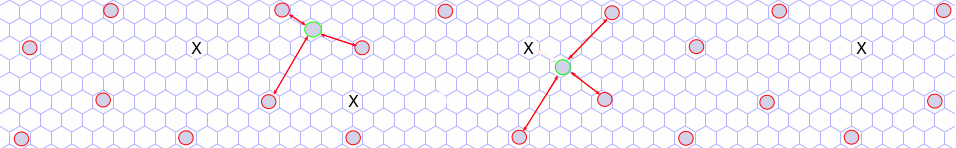
\includegraphics[scale=.45]{./figures/hex-train-disembark.png}
	\caption{Train car with the cells of disembarking passengers marked with ``X''}
	\label{social-distance-disembark}
\end{figure}

If there were more than $24$ passengers in a train car, and after all the passengers have disembarked, there are now fewer than $24$ passengers in the train car, we will re-position the remaining passengers to optimally social distance themselves as shown in Figure \ref{social-distance-full-grid} before embarking any new passengers from the station.
This behavior matches the observed behavior of subway riders.
When an packed car arrives at a popular station and many passengers disembark, the remaining passengers will re-arrange themselves to social distance to the best of their ability.
See Figure \ref{social-distance-rearrange} for an example of this rearrangement. 

\begin{figure}[h]
	\centering
	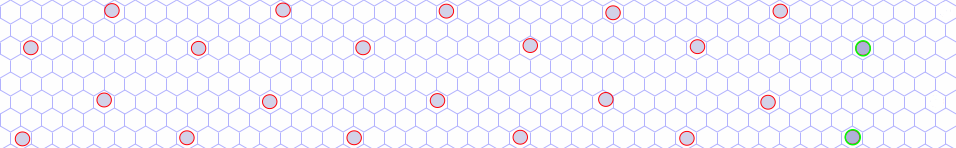
\includegraphics[scale=.45]{./figures/hex-train-rearranged.png}
	\caption{Train car with passengers rearranging to a safe configuration after Figure \ref{social-distance-disembark}}
	\label{social-distance-rearrange}
\end{figure}

Once a train at a station has had its passengers disembark, the passengers queued at the station being to embark.
Passengers will sequentially embark one at a time from the station's queue until either the queue is empty or all the train cars are full.
Each passenger from the queue will board the train car with the least occupancy at the time the passenger embarks.
When selecting a hex cell for the embarking passenger to occupy, if there are fewer than $24$ passenger within the train car, then the embarking passenger will occupy the next vacant ``safe space'' as shown in Figure \ref{social-distance-full-grid}.
If there are more than $24$ passengers within the train car, the embarking passenger will select one of the unoccupied hex cells uniformly at random.

\subsection{Virus Spread}

	\begin{figure}[h]
	\centering
	\begin{minipage}{0.32\textwidth}
		\centering
		\caption{Passengers at $t_i$}
		\label{Fig:tranmission-t_i}
		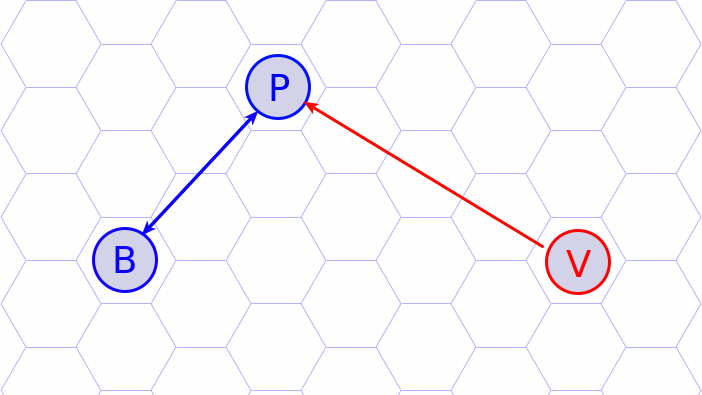
\includegraphics[width=0.95\textwidth]{./figures/hex-grid-trans-0.png}
	\end{minipage}
	\hfill
	\begin{minipage}{0.32\textwidth}
		\centering
		\caption{Passengers at $t_j$}
		\label{Fig:tranmission-t_j}
		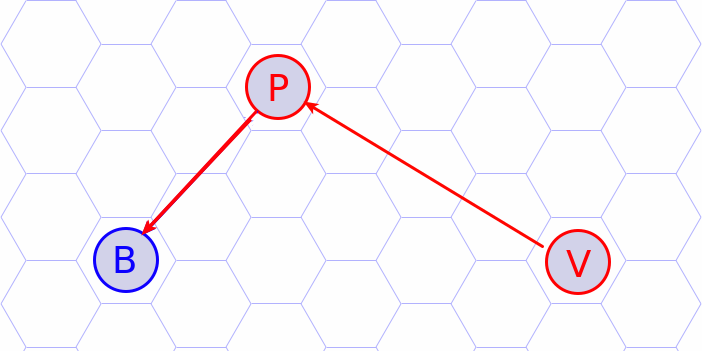
\includegraphics[width=0.95\textwidth]{./figures/hex-grid-trans-1.png}
	\end{minipage}
	\hfill
	\begin{minipage}{0.32\textwidth}
		
		\centering
		\caption{Passengers at $t_k$}
		\label{Fig:tranmission-t_k}
		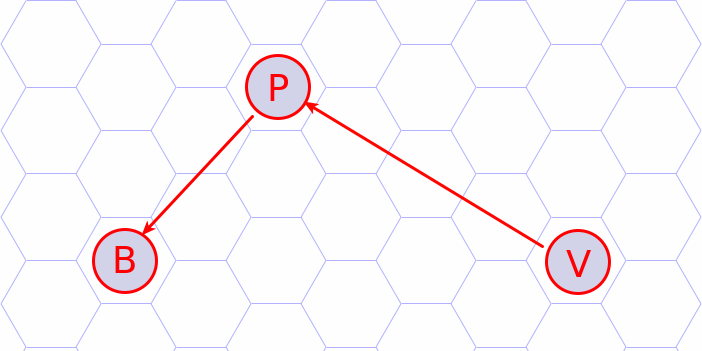
\includegraphics[width=0.95\textwidth]{./figures/hex-grid-trans-2.png}
	\end{minipage}
	
\end{figure}

Each minute that a passenger is within 4 hexes of a passenger with the virus, we call this a minute of exposure.
For each minute of exposure we increment the ``exposure time'' annotation of the passenger.
When the passenger's ``exposure time'' annotation equals or exceeds the ``time until transmission'' annotation, we consider this a novel transmission event and the passenger is annotated as having the virus.
It should be noted that if a passenger is within 4 hexes of two or more passengers with the virus, each minute of exposure is double-counted (or more) for the passenger to represent the increased risk of multiple virus transmission vectors.
For example if a passenger without the virus has a ``time to transmission'' annotation of 27 minutes, and there are \emph{four} passengers with the virus within 4 hexes of the passenger, then each minute of the simulation would increment the passenger's ``exposure time'' annotation by \emph{four}, causing the passenger to have the virus transmitted to them after 7 minutes under these simulated exposure conditions.

Our model permits the virus to spread transitively throughout the car as time advances in our simulation.
In the Figures \ref{Fig:tranmission-t_i}, \ref{Fig:tranmission-t_j}, and \ref{Fig:tranmission-t_k}, as time $t_i < t_j < t_k$, we see that the virus can be transmitted to passenger $B$ transitively from the original infected passenger $V$, through a proxy passenger $P$.
This models the real conditions of SARS-Cov-2 being able to survive on surfaces for extended periods of time and be transmitted via touch and fine particulate matter.
The virus may be transmitted to (though not infecting) a passenger and then subsequently be transmitted to another passenger in a stepping stone-like manner. 

\subsection{Randomness and Determinism}

Our project allows specifying a seed for the pseudorandom number generator (RNG) which will cause the random events within the simulation to be deterministic.
We achieve this by first seeding the global RNG.
Next, we sample a random number from the global RNG and call this value \emph{origin}.
We create a new, independent RNG with the seed \emph{origin} and we call this new RNG \emph{streamGen}.
Lastly, we create an infinite stream of new RNGs, by creating new independent RNGs seeded with values from \emph{streamGen}. 
We call this infinite stream of unique, independent RNGs \emph{streamOfRNGs}.
All of the RNG initialization is computed prior to any replication of our simulation.

Each time a simulation replication is initialized, each station $S_i^q \in \mathcal{S}$ will be given a RNG from \emph{streamOfRNGs}.
Because \emph{streamOfRNGs} is deterministically initialized, each time the program is run with the same global seed, \emph{streamOfRNGs} will produce the same RNGs in the same order.
This allows us to run our simulation under with different parameter (see Section 4 below) and compare the results confident in the fact that all of the observations are based on the same random events.

\subsection{Variance Reduction}

For our study, we attempted two routes of variance reduction.

First method was through the use of antithetic variables. The fundamental concept behind this method is to choose another independent, identical, and negatively correlated random variable compared to our target variable. This defines this pair of random variables to be "antithetic" where they will have negative covariance value between them. If we create a new random variable that represents the simple average of these pairs of variables, the mean of this new random variable with be an unbiased estimator of the mean of our target variable, but with a reduced variance.

We were able to obtain the antithetic pair by running the second set of simulations with $1-U$ value instead of $U$ value for determining initial spawning of infected passengers ( where $U$ represents the uniformly distributed random variable value within the [0,1] ). In terms of the physical simulation, this translates into simulating 2 different sets of subway systems where the two differ only in the locations where the infected people spawn ( in the 2nd set, the people will spawn in an exact "opposite" configurations ). The data set acquired from average of these two simulation results will be one that is more centered and that has less variance.

Second method was through the selection of a control random variable, for which we already know the mean and variance of, and choose it in a way that it exhibits a high covariance value with our target random variable. We then define a new random variable $Z$ (difference variable) and calculate it using our target random variable and our control input variable, such that it subtracts the variance of the input control variable from the values of our target random variable, with a proportional constant of $c$.

$$ Z = Y + c(X - E(X)) $$
where Y = target random variable and X = input control variable.

From the above definition, it is evident that the expected value of $Z$ would be equal to the expected value of $X$.

In regards to our specific study, the control variable was selected to be the amount of time an individual spends being in the over-packed subway car. It can be easily seen that this variable is correlated the our target variable as novel virus transmissions only occur in over-packed subway cars where social distancing is not fully observed, and also this variable takes into account the time and the number of people within its definition, making it an optimal choice for our control variable.

\begin{figure}[h]
	\centering
	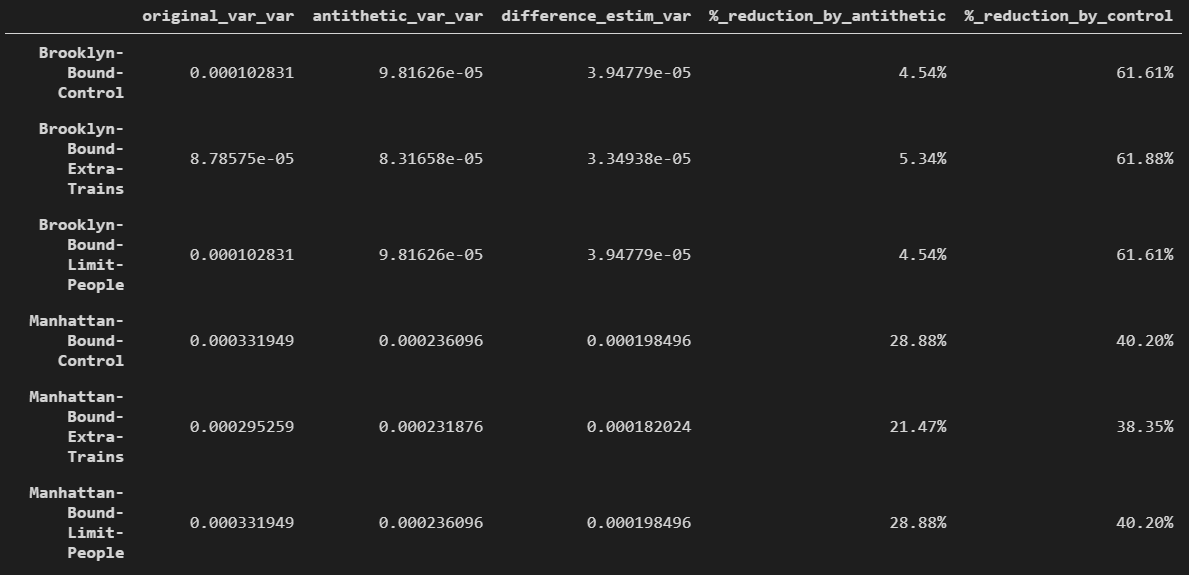
\includegraphics[scale=.42]{./figures/var-red-results.png}
	\caption{Variance Results for 6 different types of Simulation Runs \& Percent Reduction shown by 2 variance reduction methods}
	\label{var-red-results}
\end{figure}

As you can see in Figure \ref{var-red-results}, antithetic variables method achieved a range of 4\% to 28\%, where as control variable method consistently produced higher variance reduction results from 38\% to 61\%.

\section{Hypothesis, Control, and Interventions}

\subsection{Hypothesis}

To help us study the expected ratio of novel transmission of the virus, we will test a specific hypothesis.
We will run three different simulations of the MTA's L-line, one control and two interventions, to determine how certain model parameters effect the expectation of our random variable.
We hypothesize that each intervention will decrease the expectation or our model's random variable.
The implication of our hypothesis being supported by the simulations is that implementing the public policies corresponding to the intervention will reduce the transmission of SARS-CoV-2.

\subsection{Control Simulation Parameters}

For the control simulation we will as closely as possible specify parameters to our model which reflect the current MTA operations of the L-line.
To do so we specify the parameters below.
The following parameters will remained fixed between the control simulation and the interventions: $c$, $r$, $n$, $T$, $\Psi$, $\mathcal{S}$, $\Lambda$, and $M$.
The each of the parameters $q$ and $\tau$ will be allowed to vary independently in the interventions.
For the control, the maximum queue length $q$ for each station will be infinite.
This represents the MTA not taking any action to throttle the number of passengers entering the subway line.
The parameter $\tau$ will be set to the arrival times of the L line trains as advertised by the MTA's train schedule.

\begin{equation*}
\begin{split}
\text{Control}: \; c &= 0.01 \\
  r &= \frac{1}{15} \\
  n &= 24 \\
  q &= \infty \\
  T &= 1440 \\
  \Psi &= 258 \\
  \mathcal{S} &= \{ S_0^\infty, S_1^\infty, ... , S_{23}^\infty \} \\
  \Lambda &= \{ \lambda_0(t), \lambda_1(t), ... , \lambda_{23}(t) \} \\
  M &= \{ \mu_0(t), \mu_1(t), ... , \mu_{23}(t) \} \\
  \tau &= \{ t_0, t_1, ..., t_m \} \\
\end{split}
\end{equation*}


\subsection{Intervention Parameters: More Trains}

For this intervention, we consider sending train more frequently through the subway line. To do so, we modify the MTA's train schedule to use the ``rush hour'' train L-line schedule for the entire work day hours. This means that the for the time interval from \texttt{08:00} to \texttt{18:00}. trains arrive every 3-4 minutes. We modify the parameter $\tau$ of our model accordingly:

  \[ \tau = \{ t_0^{'}, t_1^{'}, ..., t_{m^{'}}^{'} \} \]

\subsection{Intervention Parameters: Fewer Passengers}

For this intervention, we consider the MTA throttling the number of passengers which can enter the subway station at a time. We will fix the number of passengers which can enter the subway station. Passengers which are rejected from entering the subway system are assumed to take alternate transportation, such as buses, ride shares, taxis, or biking. If the passenger queue at a station is full, only once the next train arrives and some of the passengers embark, can new passengers arriving at the station enter the subway system. We modify the parameter $q = 100$ of our model and update each station accordingly accordingly:

\[ \mathcal{S} = \{ S_0^{100}, S_1^{100}, ... , S_{23}^{100} \} \]


\section{Conclusions and Recommendations}
 
	We replicated our simulation $1000$ times for the control and both interventions for both the Manhattan bound and Brooklyn bound directions of the subway line. We took the mean of the random variable output from the replications. This mean value is an estimate of the expectation of the probability that a passenger without the virus entering the subway system will have the virus transmitted to them during their ride. We call this $\mathbb{E}(\mathbb{P}(spread))$. We also calculated the 95\% confidence interval for the mean in each of the six scenarios by estimating the standard deviation from the 1000 observations and using the t-value from the student's distribution. See Table \ref{main-results} for the estimated expectation of each scenario. See also Figures \ref{Fig:brooklyn-results} and \ref{Fig:manhattan-results} for a box plot visualization of the results. Not that the notched sections of the box plot depict the 95\% confidence intervals.

	The results of our simulations support the posited hypothesis. In all intervention cases, the value of $\mathbb{E}(\mathbb{P}(spread))$ decreased compared to the control. However, the degree to which the value decreased is an interesting observation. 
	
	In the Brooklyn bound cases, increasing the train arrival schedule midday had the result of decreasing $\mathbb{E}(\mathbb{P}(spread))$ by $17.6\%$. Throttling the number of passengers entering subway stations had the result of decreasing $\mathbb{E}(\mathbb{P}(spread))$ by $40.3\%$. Both these results represent a significant public health impact. 
	
	In the Manhattan bound cases, increasing the train arrival schedule midday had the result of decreasing $\mathbb{E}(\mathbb{P}(spread))$ by $3.8\%$. Throttling the number of passengers entering subway stations had the result of decreasing $\mathbb{E}(\mathbb{P}(spread))$ by $98.5\%$. The discrepancy between the efficacy of the two interventions deserves some inspection. When examining the origin-destination matrix $P_{ij}(t)$, we noticed that the values for the $P_{i(n-3)}(t)$, $P_{i(n-2)}(t)$, $P_{i(n-1)}(t)$ columns were all an order of magnitude higher than the values in the other columns. We can interpret this to mean that the majority of passengers entering the Manhattan bound subway line intent to ride the subway from Brooklyn into Manhattan to one of the last stops on the line. Because of this dynamic, the trains cars fill up faster than they empty out until the last three stops on the line. More trains running does not counter act this passenger destination preference. However, turning away passengers at the subway stations when trains are mostly full and many passengers are waiting to enter does act as an effective policy for limiting the over all train crowding.

	\begin{table}
	\centering
	\begin{tabular}{ l| c c }
		                 & $\mathbb{E}(\mathbb{P}(spread))$  & 95\% confidence interval\\
		Brooklyn Bound   & & \\
		                  \hline
		Control          & $0.00454$ & $\pm\, 0.00027;\, ( 0.00427,\;  0.00480)$ \\ 
		More Trains      & $0.00375$ & $\pm\, 0.00024;\, ( 0.00351,\;  0.00399)$ \\  
		Fewer Passengers & $0.00271$ & $\pm\, 0.00016;\, ( 0.00255,\;  0.00287)$ \\
		\\
		Manhattan Bound & & \\
		\hline
		Control          & $0.06224$ & $\pm\, 0.00071;\, ( 0.06154,\;  0.06295)$ \\ 
		More Trains      & $0.05986$ & $\pm\, 0.00070;\, ( 0.05916,\;  0.06056)$ \\  
		Fewer Passengers & $0.00090$ & $\pm\, 0.00018;\, ( 0.00072,\;  0.00108)$ \\
	\end{tabular}
	\caption{Results of our simulation}
	\label{main-results}
	\end{table}


\begin{figure}[h]
	\centering
	\caption{Brooklyn Bound Results}
	\label{Fig:brooklyn-results}
	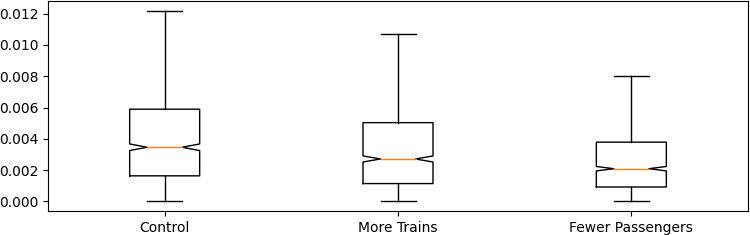
\includegraphics[width=0.95\textwidth]{./figures/brookly-bound-results.png}
\end{figure}

\begin{figure}
	\centering
	\caption{Manhattan Bound Results}
	\label{Fig:manhattan-results}
	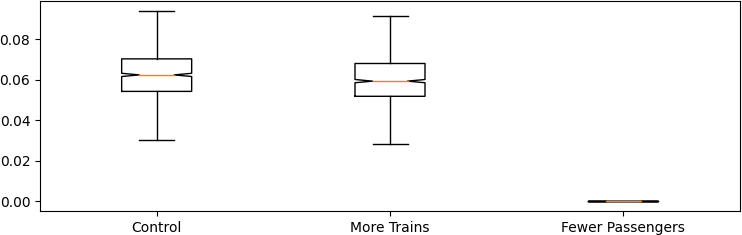
\includegraphics[width=0.95\textwidth]{./figures/manhattan-bound-results.png}
\end{figure}

\subsection {Output Analysis}

When evaluating the quality multiple simulation methods, the relevant quantity is defined as $ \sigma^{2} \tau $ where $\sigma^{2}$ represents the variance and the $\tau$ represents the time it takes to run the simulation model. The time of the Control Variable and the Original Simulation is nearly identical due to the control variable being an endogenous variable within our simulation model.

Since we have 6 different types of simulation runs, the "Manhattan-bound-Control" was selected as it showed significant performance in both variance reduction techniques. We have the following results:

\begin{center}
	\begin{tabular}{ l| c c c}
		                 & Variance      & Average Time(min) & Output Evaluation Parameter\\
		Types of V.R. techniques & & &\\
		  \hline
		Original (As-Is) & $0.000331949$ & $23$              & $0.007634827$\\ 
		Antithetic       & $0.000236096$ & $48$              & $0.011332608$\\  
		Control Variable & $0.000198496$ & $24$              & $0.004763904$\\

	\end{tabular}
\end{center}

From the Output Evaluation results, it seems that the Control Variable method shows the best performance.

\subsection {Recommendations}

We provide a strong recommendation of throttling the number of passengers entering the subway system. The first reason is the efficacy supported by our simulation. A $98.5\%$ reduction in virus transmission will have a profound public health impact. The second reason is the lower cost of implementing this policy compared to running trains more frequently. We propose the following MTA policy:

\begin{displayquote}
	Assign at least one MTA employee per set of turnstiles entering a subway line.
	Monitor the number of passengers entering each subway station via the real-time turnstile data.
	Keep a counter of the of passengers in the station visible to the MTA station staff.
	When a train departs from the station, reset the counter to 0.
	When 100 passengers have entered a station, and the counter reads 100, have the assigned MTA employees stop admitting new passengers through the turnstiles until after the next train departs and the counter has reset.
	The above represents a cost-effective policy for reducing the transmission of the virus with the subway trains by 40\% to 98\%.
\end{displayquote}

\section{General Discussion}

It is worth delving deeper into the efficacy of throttling passengers at subway stations.
It may be the case that only certain stations along the subway line need to have a throttling policy implemented and others can have no restrictions which result in the same or nearly the same efficacy.
Exploring and quantifying this would allow for an improved passenger service experience and a lower operational cost of the proposed policy.

While we emphasize the major potential for reducing virus transmission in the policy recommendation, we have not fully quantified the cost of implementing such a policy.
It is (safely) assumed that assigning MTA employees to handle turnstile admittance would be less costly than running train more frequently, we do not know the exact cost of assigning these staff members.
The number of required employees would be contingent on future research determining the minimum station at which passenger throttling would need to be implemented to reduce the virus transmission.
Furthermore, there may be capital requirements in order th facility the MTA employee's ability to monitor real-time turnstile data and reset the ``queue counter'' when trains depart.
Lastly, there is an opportunity cost when turning away passengers after the station is at capacity, each passenger not admitted represents a potential loss of fare (currently \$2.75).
We do not assume that in reality all passenger which are denied immediate access to the subway will find other transportation options.
More likely is that potential passengers will queue up outside the turnstiles and wait for admittance once the next train departs.
Some passengers may grow impatient and forego waiting in a queue outside the turnstile for access to the subway system and instead that alternative transportation, but many, perhaps even most, potential passengers are expected to wait for subway access.
To address these unresolved policy concerns, further work is required.

\subsection{Alternative Approaches and Repurposing}

During our discussions, the idea of re-purposing this simulation had come up. It wouldn't be too much work to re-purpose our model/simulation to simulate other scenarios where scheduling and social distancing is required, such as in a restaurant or a bus route/system.

\hfill \newline
Furthermore, we can also expand our model by replicating the system to account for other lines with different arrival rates for passengers and trains. There is however a challenge in integrating multiple lines together to account for transfer of passenger from one subway line to another.

    \begin{algorithm}
	\label{Alg:pre-order}
	\caption{Main simulation loop}\label{Alg:main-loop}
	\begin{algorithmic}[1]
		\Require{$c,\,r \in [0,1] \subset \mathbb{R}$}
		\Require{$\forall t \in \tau, t \in \mathbb{N}$}
		\Require{$\forall S_i^q \in \mathcal{S}, S_i^q$ is a subway station with a queue of length $q$}
		\Require{$\mathcal{D} : \mathcal{S} \times \mathcal{S} \mapsto \mathbb{Z}$}
		\Require{$|\tau|,\, |\mathcal{S}| > 0$}
		\Ensure {A set of unique passengers annotated with whether they entered with the virus and whether they exited with the virus}
		\Function{RetrospectiveSimulation}{$c,\,$ $r,\,$ $\tau,\, \mathcal{S}$}
		
		\State $\textit{departedPassengers} \gets \emptyset$
		\State $\textit{clock} \enskip \gets 0$ 
		\While{$\tau \not = \emptyset$}
		  \State $\textit{arrival} \gets$ \Call{Pop}{$\tau$}
		  \State $\textit{elapsed} \gets \textit{arrival} - \textit{clock}$
		
		  \ForEach{$S_i^q \in \mathcal{S}$} \Comment{Mutate station queues based on time between trains}
		    \State \Call{GeneratePassengersAtStation}{$\textit{clock}$, $\textit{elapsed}$, $S_i^q$}
		  \EndFor
		  
		  \State $\textit{clock} \gets \textit{clock}\; + \textit{elapsed}$
		  
		  \State $\textit{train} \gets$ \Call{ConstructEmptyTrain}{}
		
  		  \ForEach{$S_i^q \in \mathcal{S}$} \Comment{Move the train through the subway line}
  		    \State $\textit{departingPassengers} \gets$ \Call{ArriveAtStation}{$\textit{train}$, $S_i^q$}
  		    \State $\textit{departedPassengers} \gets \textit{departedPassengers} \cup \textit{departingPassengers}$
  		    \State $\textit{passengersToLoad} \gets$ \Call{GetQueue}{$S_i^q$}
  		    
  		    \While{$\textit{passengersToLoad} \not = \emptyset$}
  		      \State $\textit{passenger} \gets$ \Call{Pop}{$\textit{passengersToLoad}$}
  		      \If{\Call{AddPassenger}{$\textit{train}$, $\textit{passenger}$}}
  		      	\State \textbf{Continue}
  		      \Else \Comment{Train was full, passenger could not board train}
  		        \State \Call{Push}{$\textit{passengersToLoad}$, $\textit{passenger}$}
  		        \State \textbf{Break}
  		      \EndIf
  		    \EndWhile
  		    \State $\textit{timeToNextStation} \gets \mathcal{D}(S_i^q,S_{i+1}^q)$
  		    \State \Call{ComputePassengerTransmission}{$\textit{train}$, $\textit{timeToNextStation}$}
  		  \EndFor
  		  
		\Return $\textit{departedPassengers}$
		\EndWhile
		\EndFunction
	\end{algorithmic}
\end{algorithm}


\clearpage
\begin{thebibliography}{00}

\bibitem{Ross:2010} Ross. S.~ (2010) {\em Simulation}, Academic Press, NY.

\bibitem{tomacs-MVD}  B.~Heidergott, G.~Pflug and F.J.~V\'azquez-Abad, and and T. Farenhorst-Yuan (2010) 
``Gradient Estimation for Discrete Event Systems'',  {\em ACM-Transactions on Modeling and Computer Simulation},  vol. 20, issue 1, article  No.~5,  (28 pages).

 \bibitem{deds03_metro}    F.J.~V\'azquez-Abad and L.~Zubieta (2005) ``Ghost simulation model for
the optimisation of an urban subway system'', {\em DEDS Journal}, {\bf vol 15}, No.3.

\bibitem{mta} NYC MTA ``Day-by-day ridership numbers``,  \url{https://new.mta.info/coronavirus/ridership}

\bibitem{ridership_census} U.S. Census ``Sex Of Workers By Means Of Transportation To Work For Workplace Geography``, \url{https://data.census.gov/cedsci/table?q=ACSDT1Y2017.B08406&g=1600000US3651000&tid=ACSDT1Y2017.B08406}

\bibitem{distancing_recommendations} Chu, D. K., Akl, E. A., Duda, S., Solo, K., Yaacoub, S., Schünemann, H. J., Chu, D. K., Akl, E. A., El-harakeh, A., Bognanni, A., Lotfi, T., Loeb, M., Hajizadeh, A., Bak, A., Izcovich, A., Cuello-Garcia, C. A., Chen, C., Harris, D. J., Borowiack, E., … Schünemann, H. J. (2020). Physical distancing, face masks, and eye protection to prevent person-to-person transmission of SARS-CoV-2 and COVID-19: a systematic review and meta-analysis. The Lancet, 395(10242), 1973–1987. https://doi.org/10.1016/s0140-6736(20)31142-9

\bibitem{body_size} Fryar CD, Kruszon-Moran D, Gu Q, Ogden CL. Mean Body Weight, Height, Waist Circumference, and Body Mass Index Among Adults: United States, 1999-2000 Through 2015-2016. Natl Health Stat Report. 2018 Dec;(122):1-16. PMID: 30707668.

\bibitem{dimensions} R143 Train Car \url{https://www.kawasakirailcar.com/R143}

\bibitem{disease_numbers} NYC, ``COVID-19: Data`` \url{https://www1.nyc.gov/site/doh/covid/covid-19-data.page}

\bibitem{viral_load} Carl Heneghan, Jon Brassey, Tom Jefferson ``SARS-CoV-2 viral load and the severity of COVID-19``\url{https://www.cebm.net/covid-19/sars-cov-2-viral-load-and-the-severity-of-covid-19/}

%\bibitem{guangzhou-study} Luo, L., Liu, D., Liao, X., Wu, X., Jing, Q., Zheng, J., Liu, F., Yang, S., Bi, H., Li, Z. and Liu, J., 2020. Contact settings and risk for transmission in 3410 close contacts of patients with COVID-19 in Guangzhou, China: a prospective cohort study. Annals of internal medicine.

\bibitem{arrival_rate} MTA Turnstile Data \url{http://web.mta.info/developers/turnstile.html}

\end{thebibliography}

\end{document}